

% use `pdflatex -shell-escape Perfect_Circumplex.tex` in the terminal

\documentclass[border={25pt 25pt 25pt 25pt},tikz,convert={outext=.svg,command=\unexpanded{pdf2svg \infile\space\outfile}},multi=false]{standalone}

%\documentclass[border={25pt 25pt 25pt 25pt}]{standalone}
\usepackage[utf8]{inputenc}
\usepackage{todonotes}
\usetikzlibrary{decorations.pathmorphing, decorations.text}
\renewcommand{\familydefault}{\sfdefault} 



\begin{document}
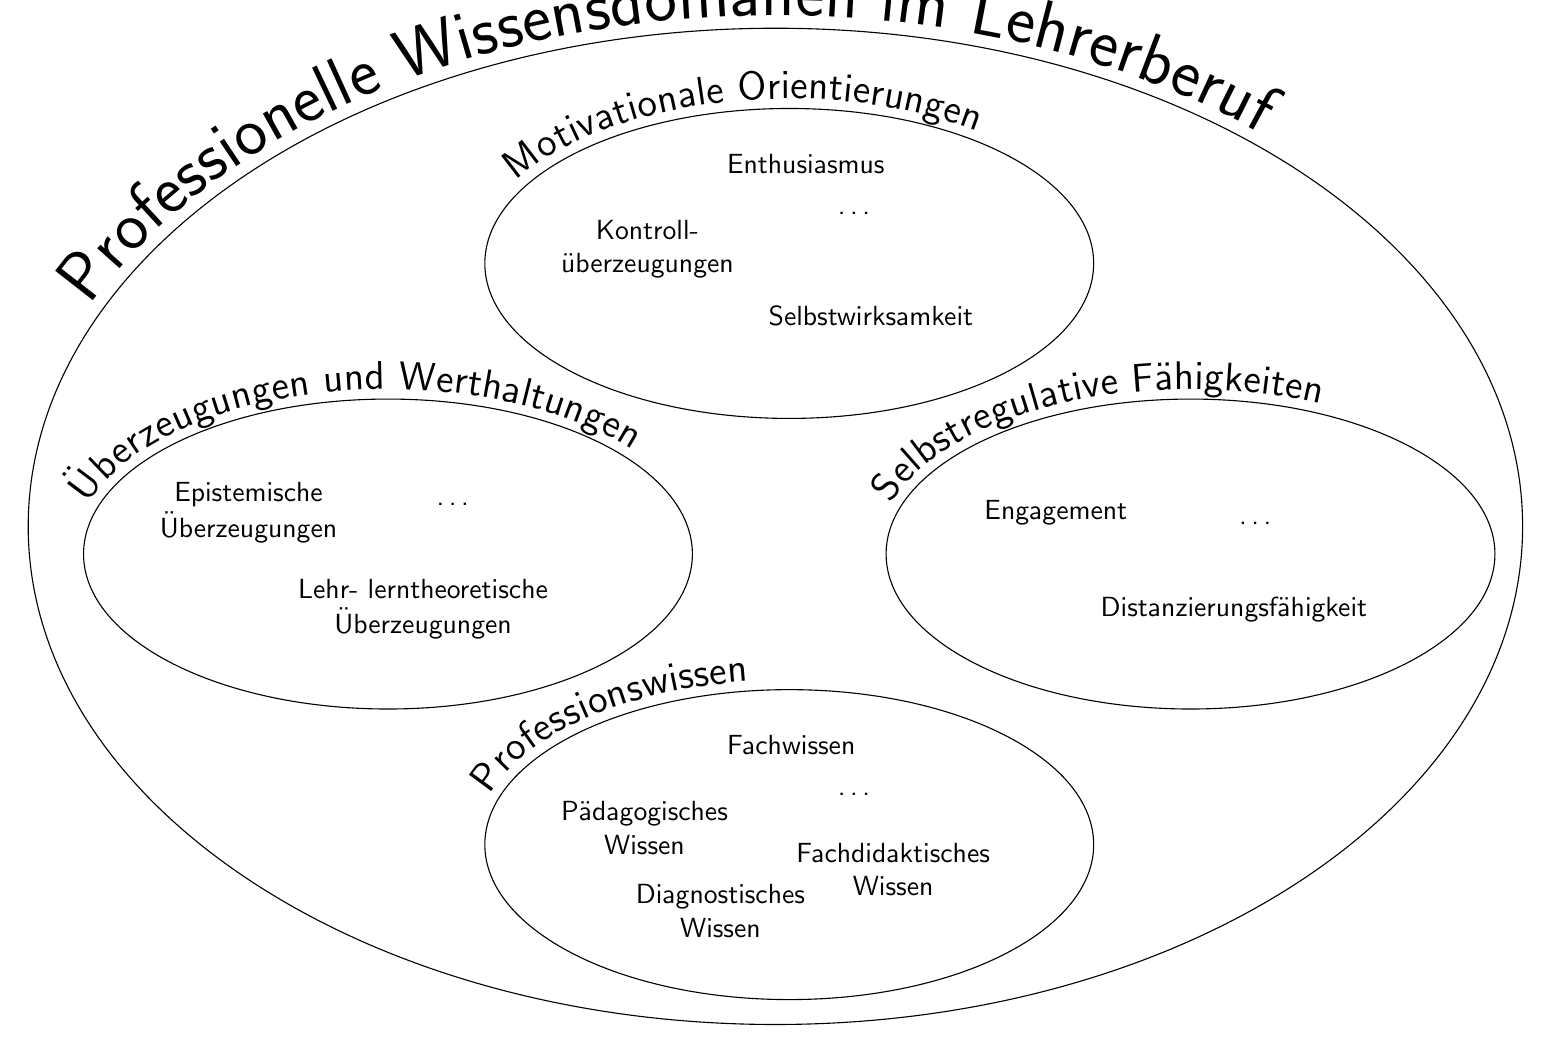
\begin{tikzpicture}


\draw[rotate=0,
 postaction={decorate,
    decoration={raise=.45em, 
    text along path, pre length=28cm,
      text={|\Huge|Professionelle Wissensdom{ä}nen im Lehrerberuf},
    },
  }] (0,0) arc (360:0:270pt and 180pt);  
  
  
 \draw[rotate=0,
 postaction={decorate,
    decoration={raise=.35em, 
    text along path, pre length=10cm,
      text={|\Large|Professionswissen},
    },
  }] (-155pt,-115pt) arc (360:0:110pt and 56pt);  % Große Ellipse 270 breit --> 
  

 \draw[rotate=0,
 postaction={decorate,
    decoration={raise=.35em, 
    text along path, pre length=10.5cm,
      text={|\Large|Motivationale Orientierungen},
    },
  }] (-155pt,+95pt) arc (360:0:110pt and 56pt);  % Große Ellipse 270 breit --> 
  
  
 \draw[rotate=0,
 postaction={decorate,
    decoration={raise=.35em, 
    text along path, pre length=10cm,
      text={|\Large|Selbstregulative F{ä}higkeiten},
    },
  }] (-10pt,-10pt) arc (360:0:110pt and 56pt);  % Große Ellipse 270 breit --> 
    

 \draw[rotate=0,
 postaction={decorate,
    decoration={raise=.35em, 
    text along path, pre length=10cm,
      text={|\Large|{Ü}berzeugungen und Werthaltungen},
    },
  }] (-300pt,-10pt) arc (360:0:110pt and 56pt);  % Große Ellipse 270 breit --> 
   

%% Inhalte Überzeugungen %%%%%%%%%%%%%%%%%%%%%%%
\draw (-470pt,5pt) node [text width=2cm]{  
  \begin{tabular}{c}
    Epistemische\\ Überzeugungen
  \end{tabular}};
  
%% Labels
\draw (-420pt,-30pt) node [text width=2cm]{  
  \begin{tabular}{c}
    Lehr- lerntheoretische\\ Überzeugungen
  \end{tabular}};
  
%% Labels
\draw (-370pt,10pt) node [text width=2cm]{  
  \begin{tabular}{c}
     \dots 
  \end{tabular}};

%% Inhalte Professionswissen %%%%%%%%%%%%%%%%%%
\draw (-325pt,-110pt) node [text width=2cm]{  
  \begin{tabular}{c}
    Pädagogisches\\Wissen
  \end{tabular}};
  
%% Labels
\draw (-265pt,-80pt) node [text width=2cm]{  
  \begin{tabular}{c}
    Fachwissen
  \end{tabular}};
  
%% Labels
\draw (-225pt,-95pt) node [text width=2cm]{  
  \begin{tabular}{c}
     \dots 
  \end{tabular}};

\draw (-240pt,-125pt) node [text width=2cm]{  
  \begin{tabular}{c}
    Fachdidaktisches\\Wissen
  \end{tabular}};

\draw (-298pt,-140pt) node [text width=2cm]{  
  \begin{tabular}{c}
    Diagnostisches \\Wissen
  \end{tabular}};

%% Inhalte Motivationale Orientierungen %%%%%%%%%%%%%%%%%%
\draw (-325pt,100pt) node [text width=2cm]{  
  \begin{tabular}{c}
    Kontroll-\\überzeugungen
  \end{tabular}};
  
%% Labels
\draw (-265pt,130pt) node [text width=2cm]{  
  \begin{tabular}{c}
    Enthusiasmus
  \end{tabular}};
  
%% Labels
\draw (-225pt,115pt) node [text width=2cm]{  
  \begin{tabular}{c}
     \dots 
  \end{tabular}};

\draw (-250pt,75pt) node [text width=2cm]{  
  \begin{tabular}{c}
    Selbstwirksamkeit
  \end{tabular}};
  
%% Inhalte Selbstregulative %%%%%%%%%%%%%%%%%%%%%%%
\draw (-172pt,5pt) node [text width=2cm]{  
  \begin{tabular}{c}
    Engagement
  \end{tabular}};
  
%% Labels
\draw (-130pt,-30pt) node [text width=2cm]{  
  \begin{tabular}{c}
    Distanzierungsfähigkeit
  \end{tabular}};
  
%% Labels
\draw (-80pt,3pt) node [text width=2cm]{  
  \begin{tabular}{c}
     \dots 
  \end{tabular}};  


\end{tikzpicture}
\end{document}
